\chapter{Propuesta de solución}\label{chapter:proposal}

Este capítulo introduce una propuesta para enfrentar el reto de clasificar de manera automática el cáncer de piel, empleando técnicas de aprendizaje profundo. La solución se centra en la utilización de una red neuronal profunda pre-entrenada, combinada con un algoritmo propio para el ajuste de precisión.

En el núcleo de la estrategia se encuentra el uso de una red neuronal convolucional pre-entrenada EfficientNetB1. Esta red, desarrollada a partir de extensos conjuntos de datos y experiencias previas, ofrece una base sólida y rica en características para nuestro modelo. Al aprovechar este pre-entrenamiento, se puede acelerar significativamente el proceso de aprendizaje del modelo, al tiempo que aumentamos su capacidad para generalizar y reconocer patrones complejos en las imágenes dermatoscópicas.

Para complementar el enfoque metodológico, se seleccionan un conjunto de herramientas tecnológicas avanzadas. Estas herramientas están diseñadas para optimizar el rendimiento del modelo, mejorar la precisión de la clasificación y garantizar una implementación efectiva. Entre ellas, destaca una capa de normalización, una capa densa, una de regularización, una de \textit{dropout} y una de salida (capa densa con activación \textit{softmax}). Estas técnicas le permiten al modelo afinar su capacidad de identificar con precisión las diferentes categorías de lesiones cutáneas.

\section{Desarrollo del modelo y estrategias de optimización}\label{sec:method}
%-----------------------------------------------------------------------------------

Para abordar efectivamente el desafío de la detección de cáncer de piel, se seleccionó la arquitectura EfficientNetB1 \brackcite{efficientnet} como base del modelo. Esta red neuronal convolucional, parte de la familia EfficientNet, se caracteriza por su alta eficiencia y precisión. Utilizando un modelo pre-entrenado, se aprovecharon los pesos derivados de conjuntos de datos extensos, lo que facilitó la adaptación del modelo al conjunto de datos específico \brackcite{tan2019efficientnet}.

\subsection{Arquitectura del modelo EfficientNet}
   
La familia de arquitecturas EfficientNet \brackcite{tan2019efficientnet}, surgió con el objetivo de hallar un método adecuado para escalar las CNNs de manera que mejoraran tanto en precisión (i.e., rendimiento del modelo) como en eficiencia (es decir, en términos de parámetros del modelo y FLOPS). 

Inicialmente, el enfoque se centraba en aumentar la profundidad o el ancho de la red. Sin embargo, este método de escalado único tenía limitaciones y no se comprendía completamente. La investigación de EfficientNet reveló que un escalado uniforme en todas las dimensiones de la red (profundidad, ancho y resolución) usando un conjunto de coeficientes de escalado fijos podría lograr un mejor equilibrio y rendimiento. Este enfoque innovador, denominado escalado compuesto, aborda el problema del escalado en ConvNets de manera integral. Los resultados empíricos mostraron que escalar cualquier dimensión de la red mejora la precisión, pero el beneficio disminuye en modelos más grandes. Por lo tanto, se propuso un método de escalado que coordina y equilibra estas dimensiones, en lugar de escalar una sola dimensión a la vez.

EfficientNet comenzó con la creación de un modelo base, EfficientNet-B0, utilizando una búsqueda de arquitectura neural multiobjetivo que optimizaba tanto la precisión como los FLOPS. Esta red base se caracterizaba por su bloque principal, el cuello de botella móvil invertido \textit{MBConv}, y la optimización de compresión y excitación. El proceso de escalado de EfficientNet se realizó en dos etapas principales. Primero, se fijaron ciertos parámetros y luego se escaló la red base para obtener variantes más grandes, desde EfficientNet-B1 hasta B7, utilizando el método de escalado compuesto. Mientras que la arquitectura EfficientNet B0 tiene $5.3$ millones de parámetros y acepta imágenes de entrada de $224x224$, EfficientNet B7 cuenta con $66$ millones de parámetros y acepta imágenes de $600x600$ \brackcite{Tan2019EfficientNetRM}.
  
   \begin{figure}[H]
      \begin{center}
      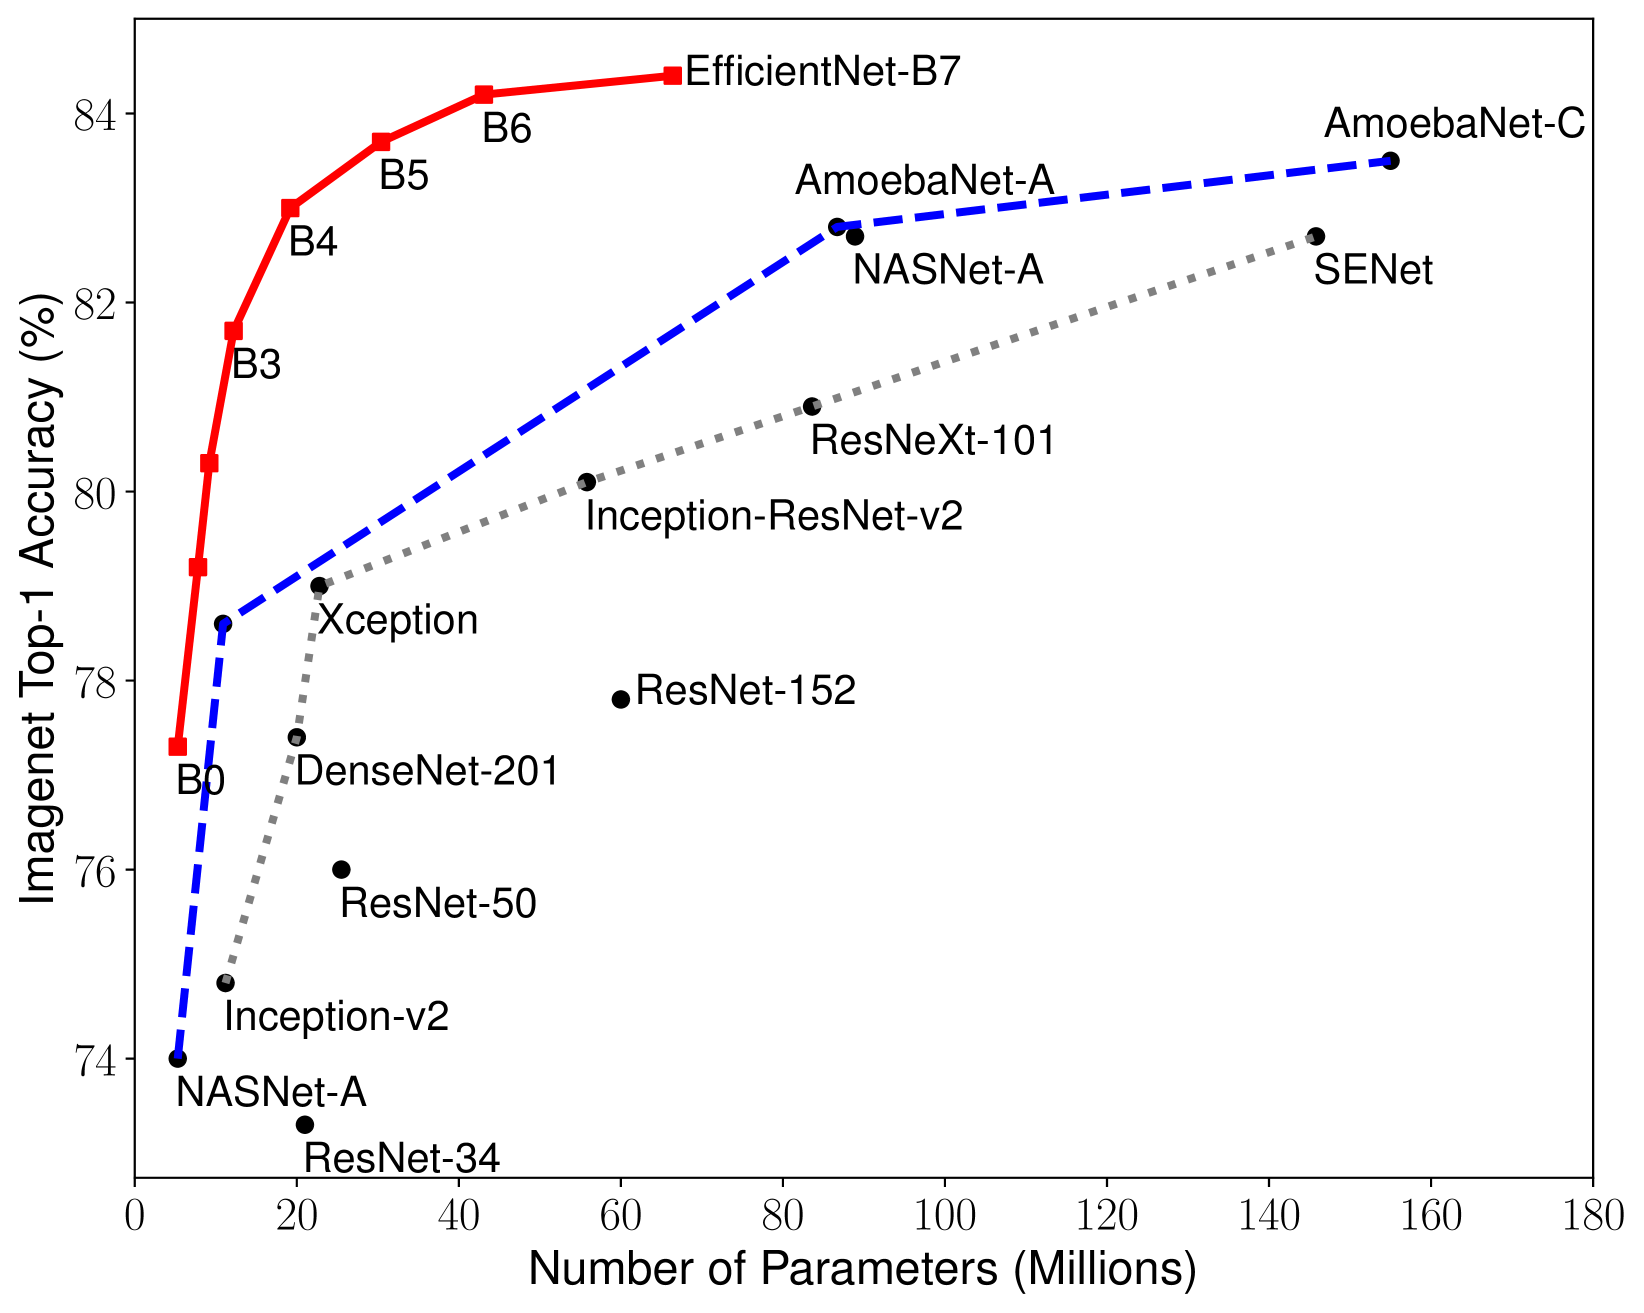
\includegraphics[width=1\textwidth]{./Graphics/efficientnet_performance.png}
      \caption{Estadísticas del rendimiento de los modelos de EfficientNet \brackcite{tan2019efficientnet}.}
      \label{fig:efficientnet_performance}
      \end{center}
      \end{figure}

Los experimentos demostraron que el método de escalado compuesto mejoraba la precisión en modelos ya existentes como MobileNets y ResNet. Los modelos EfficientNet entrenados en ImageNet mostraron una precisión y eficiencia significativamente mayores en comparación con otros ConvNets, utilizando una cantidad mucho menor de parámetros y FLOPS. Especialmente, EfficientNet-B7 logró una precisión del 84.3\% en top-1 en ImageNet, superando modelos anteriores y siendo considerablemente más pequeño y rápido.

La implementación del EfficientNetB1 puede ser particularmente beneficiosa para el análisis de datos. Este entre las variantes de la serie EfficientNet, se encuentra en un punto medio en términos de complejidad y tamaño, ofreciendo un equilibrio entre precisión y eficiencia computacional.

\section{Diseño y entrenamiento del modelo}

El modelo EfficientNetB1 se carga pre-entrenado con pesos de \textit{ImageNet} \brackcite{Pinecone2021ImageNet}, una amplia base de datos de imágenes ampliamente utilizada para entrenamiento y \textit{benchmarking} en visión por computadora. Luego a este se le omitió la capa superior para permitir la incorporación y personalización de capas adicionales. 

Luego que \textit{efficientnet} extrae las características relevantes se obtiene un vector de características. Este vector se normaliza mediante la capa de \textit{Batch Normalization}, ajustando los valores a una escala manejable y estabilizando el entrenamiento. El vector normalizado se introduce en una capa densa. En esta capa cada neurona calcula una suma ponderada de sus entradas, aplica regularizadores si están activos, y luego utiliza la función de activación \textit{ReLU}, que convierte los valores negativos a 0 y mantiene los positivos. Durante el entrenamiento, se aplica \textit{dropout}, desactivando aleatoriamente una cantidad de neuronas en esta capa para prevenir el sobre-ajuste. La salida de  la capa \textit{Dropout} pasa a través de una capa densa final con 7 neuronas, una por cada clase para luego sus salidas sean convertidas en probabilidades. Luego se calcula el error comparando esta etiqueta con las probabilidades obtenidas con la salida del modelo. Ya por último el optimizador utilizado ajusta los pesos del modelo basándose en este error y con los pesos ajustados, la siguiente iteración comienza con una nueva imagen de entrada, repitiendo el proceso.

\begin{figure}[H]
   \begin{center}
   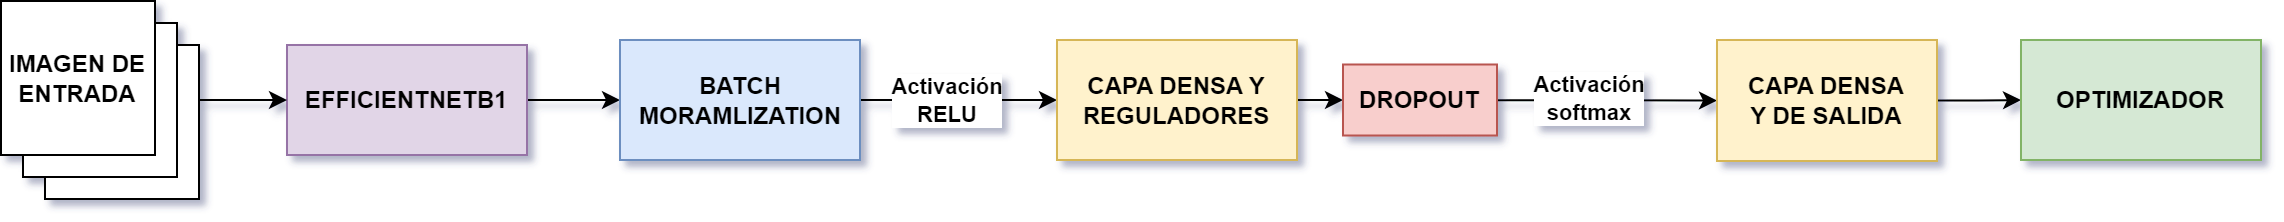
\includegraphics[width=1\textwidth]{./Graphics/diagrama_modelo.drawio.png}
   \caption{Diagrama del modelo propuesto.}
   \label{fig:model_permormance}
   \end{center}
   \end{figure}

\section{Ajuste dinámico del \textit{learning rate}}

Un elemento innovador del entrenamiento fue el uso de un \textit{callback} personalizado para el ajuste dinámico del \textit{learning rate} \brackcite{lr}. Se implementa un mecanismo de ajuste de la tasa de aprendizaje (LRA) personalizado. Este, ajusta dinámicamente la tasa de aprendizaje durante el entrenamiento basado en la precisión y la pérdida de validación, con el objetivo de mejorar la eficiencia del entrenamiento y alcanzar una mejor convergencia. Los componentes clave del LRA son:

\begin{enumerate}
   \item Modelo: La red neuronal sobre la que se aplicará el \textit{callback}.
   \item Paciencia: El número de épocas que se esperará sin mejora en la métrica de rendimiento antes de realizar un ajuste.
   \item Umbral (\textit{Threshold}): Un valor límite que define cuándo se considera que ha habido una mejora significativa en el rendimiento.
   \item Factor de Ajuste: La magnitud por la cual se modificará el \textit{learning rate} en caso de no observarse mejoras.
   \item Dwell: Una opción que permite al modelo volver a un estado de pesos anterior si no hay mejoras tras el ajuste del \textit{learning rate}.
\end{enumerate}

La clase LRA se inicializa con varios parámetros, incluyendo la paciencia para ajustar y detener el entrenamiento, el umbral para cambiar entre monitorear la precisión o la pérdida, y factores para ajustar la tasa de aprendizaje. También guarda los pesos iniciales del modelo obtenidos de la red neuronal pre-entrenada. Durante el entrenamiento, el \textit{callback} monitorea constantemente el rendimiento del modelo en términos de precisión y pérdida de validación. Este obtiene la precisión del entrenamiento, la precisión de validación, la pérdida de entrenamiento y la pérdida de validación y se va ajustando de la siguiente forma: si la precisión del entrenamiento es menor que el umbral, ajusta la tasa de aprendizaje basándose en la precisión del entrenamiento. De lo contrario, utiliza la pérdida de validación. Si hay mejoría (según la métrica monitoreada), guarda los mejores pesos y reinicia los contadores de paciencia. Si no hay mejoría durante un número de épocas igual a patience, ajusta la tasa de aprendizaje multiplicándola por un \textit{factor}. Además el mismo comprueba si \textit{dwell} es verdadero, de ser así restablece los pesos a los mejores pesos anteriores. Por cada iteración se imprime el estado actual del entrenamiento, incluyendo la tasa de aprendizaje y la métrica monitoreada. Si la tasa de aprendizaje se ha ajustado \textit{stop\_patience} veces sin mejora, detiene el entrenamiento prematuramente evitando el sobre-ajuste.

\begin{figure}[H]
   \begin{center}
   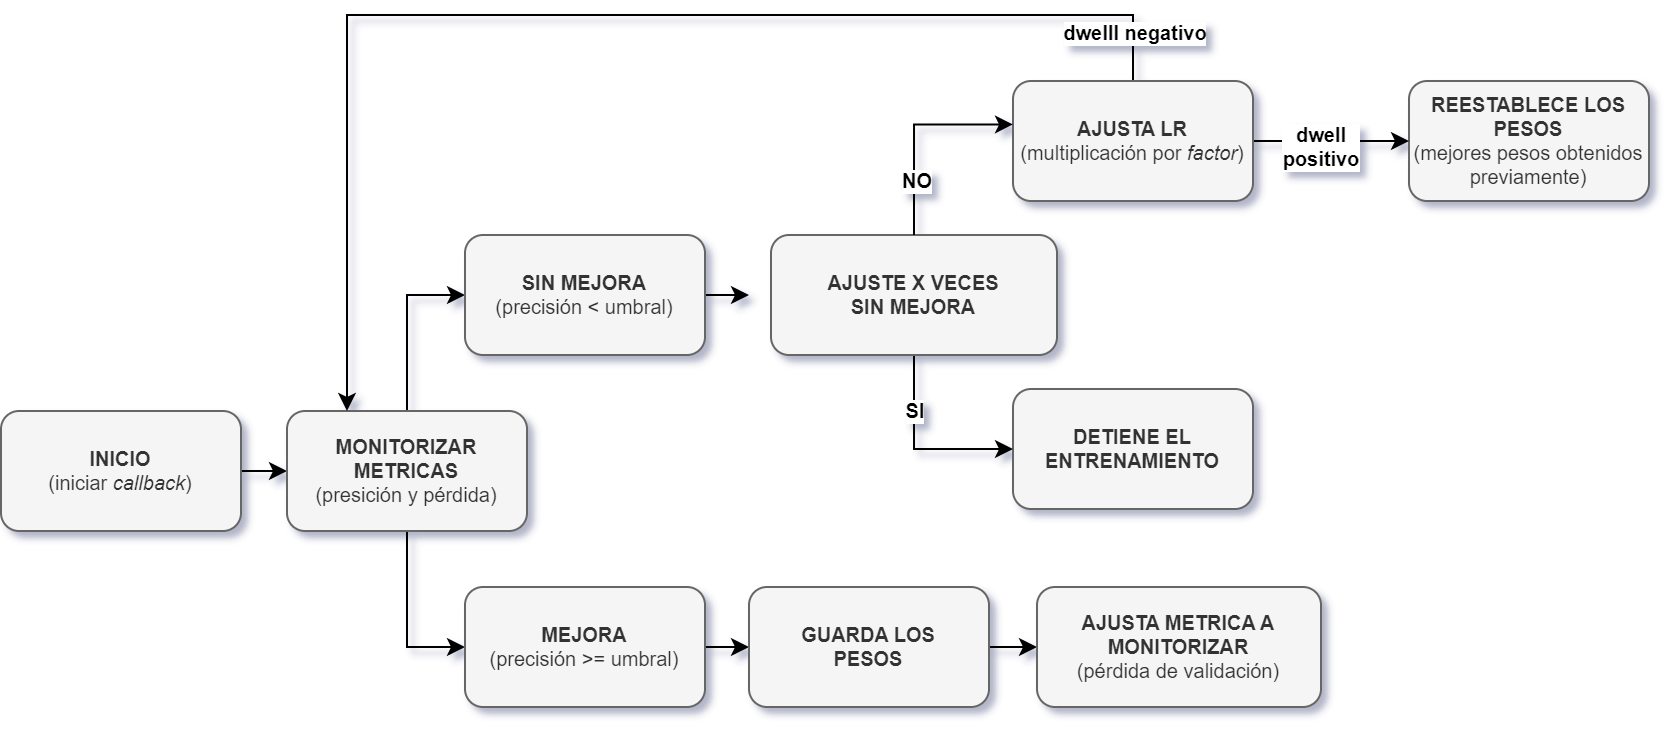
\includegraphics[width=0.85\textwidth]{./Graphics/diagrama_lra.drawio.png}
   \caption{Diagrama del ajuste dinámico de la tasa de aprendizaje.}
   \label{fig:lra_permormance}
   \end{center}
   \end{figure}

Las métricas utilizadas para la evaluación del modelo que se imprimen en cada iteración se describen en la siguiente tabla:

\begin{table}[H]
   \centering
   \small
   \begin{tabular}{|c|p{10cm}|}
   \hline
   \textbf{Término} & \textbf{Descripción} \\
   \hline
   Epoch & Es una iteración completa sobre todo el conjunto de datos de entrenamiento. \\
   \hline
   Loss (Pérdida) & Es una medida de cuán bien el modelo está realizando sus predicciones. Los valores decrecientes indican una mejora en el aprendizaje. \\
   \hline
   Accuracy (Precisión) & Muestra el porcentaje de etiquetas que el modelo predice correctamente para el conjunto de entrenamiento. \\
   \hline
   V loss (Pérdida de Validación) & Es similar a la pérdida, pero se calcula sobre un conjunto de datos que no se utiliza para el entrenamiento. \\
   \hline
   V acc (Precisión de Validación) & Muestra el porcentaje de etiquetas que el modelo predice correctamente para el conjunto de datos de validación. \\
   \hline
   LR (Learning Rate) & La tasa de aprendizaje dicta cuánto se ajustan los pesos del modelo en cada actualización. \\
   \hline
   Next LR (Próxima Learning Rate) & Indica la próxima tasa de aprendizaje planificada. La adaptación de la tasa de aprendizaje puede ayudar a evitar el estancamiento y mejorar la convergencia. \\
   \hline
   Monitor & Muestra la métrica que se está utilizando para monitorizar el rendimiento del modelo. Cambia de \textit{accuracy} a \textit{val loss}, lo que probablemente indica que el cambio se hizo para evitar el sobre'ajuste. \\
   \hline
   Duration (Duración) & Tiempo que tardó cada epoch en completarse. Importante para evaluar la eficiencia del entrenamiento. \\
   \hline
   \end{tabular}
   \caption{Descripción de términos clave en el entrenamiento de modelos de aprendizaje automático.}
   \label{table:terminology}
   \end{table}

Para la evaluación final del modelo se utilizan las métricas descritas anteriormente, matrices de confusión, gráficos sobre errores en clases, gráficos de precisión y pérdida e informes de clasificación.